\label{sec:daemon}
%\subsection{Motivation} % Jens
Wie schon erwähnt, ist eines unserer Ziele, Tweets von Twitter zu bestimmten Suchbegriffen, bei uns \textit{search terms} genannt, zu sammeln und weiterzuverarbeiten.
Da wir aufgrund einiger Restriktionen durch Twitter nicht direkt alle Tweets zu einem Thema bekommen können, ist es notwendig sie zwischenzuspeichern.
Der Service, der die Tweets von Twitter abruft und in der lokalen Datenbank speichert, wurde in Anlehnung an Unix-Dienste 
%(siehe dazu \url{https://de.wikipedia.org/wiki/Daemon}) 
Daemon genannt. 
Im folgenden Kapitel \ref{sssection:twitter-api} wird auf die Twitter-API sowie  die damit verbundenen Restriktionen eingegangen.
Anschließend wird in Abschnitt \ref{ssection:Suchstrategie} erklärt, wie die Tweets von Twitter abrufen  werden und insbesondere welche Suchstrategie dabei angewendet wird, um möglichst alle Tweets zu einem Thema zu finden.
Es folgt in Abschnitt \ref{ssection:parallele-suche} eine Beschreibung der Erweiterung der Suche zur parallelen Suche, um den Durchsatz der gefundenen Tweets zu erhöhen.
In diesem Rahmen wird auch das mit der Suche eingeführte Multi-Threading erläutert.
Als letzte Verbesserung des Daemon folgt in Abschnitt \ref{ssection:ZeitnaheErgebnisse} die Erläuterung wie möglichst zeitnah nach Eingabe eines neuen Suchbegriffs Ergebnisse erhalten werden.
Als letztes folgt im Abschnitt \ref{ssection:ausblick} eine Diskussion über 
weitere mögliche Erweiterungen der Fähigkeiten des Daemon, die nicht mehr umgesetzt werden konnten.
Das Sentiment wird zwar im Daemon berechnet, wird aber nicht hier beschrieben, sondern in Kapitel \ref{sec:Sentiment}, welches speziell nur das Thema Sentiment behandelt.

\subsection{Twitter-API}
\label{sssection:twitter-api}
Die Twitter-API umfasst alle Möglichkeiten über die zum Teil unterschiedlichen offiziellen Schnittstellen mit Twitter zu interagieren.
Sie bildet alle Funktionen ab, die notwendig sind, um einen Twitter-Client zu bauen.
Um die API verwenden zu können, benötigt man sowohl ein sogenanntes Profil, d.\,h. einen Account bei Twitter, als auch einen API-Key, den man selbst erzeugen kann.
Twitter unterscheidet zwischen dem sogenannten \textit{consumer key}, der an das Profil gebunden ist, und dem \textit{application key}, der an die Anwendung gebunden ist.
Dabei kann ein Nutzer verschiedene Apps nutzen, die alle einen eigenen \textit{application key} nutzen, sein \textit{consumer key} ändert sich aber nicht.
Genauso kann ein Entwickler mehrere Apps entwickeln, die alle einen unterschiedlichen \textit{application key} besitzen, sein \textit{consumer key} bleibt aber gleich.
Ein Nutzer muss bei einer App allerdings nicht selbst diese Keys eintragen, vielmehr fordert die App, die den \textit{application key} im Code enthält, den User auf, die App bei Twitter zu autorisieren.
Die Details lassen sich in der Twitter-Dokumentation, Abschnitt "`Access Token"' \cite{TwitterAccessTokens2014} entnehmen.
Das Authentifizierungssystem für Apps von Twitter basiert dabei auf  OAuth, auch hier finden sich wieder die Details in der Twitter-Dokumentation \cite{TwitterOAuth2014}.
Unser Daemon greift im Gegensatz dazu etwas anders auf Twitter zu.
So haben wir für jedes genutzte Profil eine eigene App bei Twitter registriert und die jeweiligen \textit{consumer} und \textit{application Keys} direkt verwendet.
Diese Art des Zugriffs ist eigentlich nur für Entwickler vorgesehen.

\subsubsection{Beschränkungen der Twitter-API}
Grundsätzlich bietet Twitter zwei unterschiedliche APIs: die REST-API und die Streaming-API. Bei der REST-API müssen explizite Anfragen gestellt  werden, um Daten zu erhalten, während bei der Streaming-API zu gewissen Themen oder Usern ständig die aktuellen Daten übermittelt werden, solange man eine Verbindung offen hält.
Die einzige für uns relevante Funktionalität ist die Suche nach den durch den Nutzer vorgegeben Begriffen, deswegen beschränken wir uns auf die Funktionalität zum Suchen nach Tweets.
Das ist grundsätzlich mit beiden APIs möglich, die Streaming-API würde es uns aber nur erlauben, Tweets zu dem gesuchten Begriff zu erhalten, die nach unserer Anfrage erstellt wurden. Das folgt aus der zweiten Grafik in der Dokumentation der Twitter Streaming-API \cite{TwitterStreamingAPIs2014}.
Es ist mit der Streaming-API also nicht möglich Tweets zu finden, die zeitlich vor Beginn unserer Anfrage erstellt wurden.
Die REST-API hingegen erlaubt es uns auch nach Tweets zu suchen, die schon vor Beginn unserer Anfrage erstellt wurden.
Allerdings gibt es auch hier  Beschränkungen.
So garantiert Twitter nicht, dass man Tweets findet, die älter als ca. 6-9 Tage sind, obwohl es durchaus ältere Tweets geben kann.
Die Dokumentation zur Nutzung der Suche \cite{TwitterUsingSearch2014} sagt dazu 
\begin{quote}
The Search API is not a complete index of all Tweets, but instead an index of recent Tweets. At the moment that index includes between 6-9 days of Tweets.
\end{quote}
Ebenfalls hier wird auch die Beschränkung erläutert, dass Twitter keine Vollständigkeit der Ergebnisse garantiert, sondern nur davon spricht, die möglichst relevanten Ergebnisse zu liefern.
Weitere Beschränkungen sind:
\begin{itemize}
\item maximal 100 Tweets pro Anfrage und
\item maximal 180 Anfragen pro 15-Minuten-Intervall pro Account (siehe \textit{REST API v1.1 Limits per window by resource} in der Twitter Dokumentation \cite{TwitterRESTLimitsperResource2014}).
\end{itemize}
Eine Einführung in diese \textit{rate limits} genannten Beschränkungen findet sich im Artikel \textit{REST API Limiting in v1.1} (\cite{TwitterRESTAPIv1.1}) der offiziellen Dokumentation.
Für uns ist außerdem noch relevant, dass Twitter es nicht ermöglicht die Suche durch kleinere Intervalle als Tage einzuschränken.
Dafür ist es möglich die Suche durch Angabe einer maximalen bzw. minimalen Tweet-ID einzuschränken.
Diese sowie weitere mögliche Parameter bei der Suche sind im \textit{GET search/tweets} Artikel \cite{TwitterSearch2014} der Twitter-Dokumentation zu finden.
Ebenfalls hier werden die \textit{result types} eingeführt.
Die \textit{result types} geben dabei an, von welcher Art das Ergebnis ist. Mögliche Werte sind:
\begin{itemize}
\item \texttt{popular} - Enthält nur die populärsten Tweets 
\item \texttt{recent} - Enthält die aktuellsten Tweets
\item \texttt{mixed} - Enthält beide Arten von Tweets
\end{itemize}
Dabei liefert der \textit{result type} \texttt{recent} nicht nur aktuelle Tweets, sondern diese auch in einer chronologischen Sortierung.
Wir konnten in eigenen Tests keine nicht-chronologische Abfolge von Tweets feststellen.
Außerdem scheint \texttt{recent} es uns zu erlauben alle Tweets zu erhalten, die Twitter uns zur Verfügung stellt.
Wir konnten jedenfalls keine fehlenden Tweets feststellen, als wir mit den verschiedenen Strategien experimentiert haben. %TODO: Beim Vergleich mit der Websiuche von Twitter
Unsere Tests erfolgten dabei unter der Annahme, dass die mit \texttt{recent} erhaltenen Tweets streng chronologisch sind.
Leider waren wir nicht in der Lage, eine genaue Aussage zur Chronologie und Vollständigkeit der verschiedenen \textit{result types} in der Twitter-Dokumentation zu finden.

\subsection{Suchstrategie} % torsten
\label{ssection:Suchstrategie}

Um Tweets von Twitter systematisch abzufragen, wird eine intelligente Suchstrategie benötigt.
Die Strategie muss sich dabei den durch Twitter auferlegten Einschränkungen anpassen.
Beispielsweise ist es mit der Search-API, die Teil der bereits erwähnten REST-API ist und für die Suche nach Tweets verwendet wird, nicht möglich, nach Tweets in Zeiträumen von Stunden oder Minuten zu suchen.
Stattdessen bietet Twitter mit der Search-API die Suche nach Tweets in Zeitintervallen von Tagen oder die Suche bis zu einer Tweet-ID an.
Letzteres bedeutet, dass eine Anfrage zu einem Suchbegriff an Twitter mit einer Tweet-ID gesendet werden kann, in der der Benutzer die 100 letzten Tweets zu diesem Suchbegriff mit einer ID kleiner als der in der Anfrage verwendeten ID erhält.

Im Daemon gab es zwei Ansätze, wie die Suche durchzuführen sein sollte.
Der erste Ansatz sah vor, dass in der ersten Phase ab dem Zeitpunkt $t$, an dem ein neuer Suchbegriff in die Datenbank geschrieben wurde, bei Twitter nach Tweets gesucht wird, die vor $t$ veröffentlicht wurden.
Werden anschließend keine neuen Tweets mehr gefunden, deren Erstelldatum vor $t$ liegt, so wird nun in einer zweiten Phase ab $t$ nach neuen Tweets gesucht.
Abbildung \ref{fig:search_1} verdeutlicht diesen Ansatz.

\begin{figure}
\centering
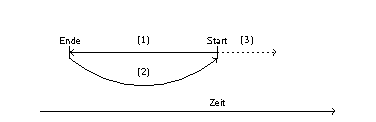
\includegraphics[width=\textwidth]{Bilder/Daemon/SearchStrategy1.pdf}
\caption{Der erste Ansatz. Zunächst wird vom Start aus rückwärts gesucht (1). Anschließend wird wieder zum ursprünglichen Start gesprungen (2). Von dort aus wird dann vorwärts nach neuen Tweets gesucht (3).\label{fig:search_1}}
\end{figure}

Der alternative Ansatz unterscheidet sich in der zweiten Phase vom ersten Ansatz.
Anstatt ab Zeitpunkt $t$ in Richtung Gegenwart zu suchen, wird der Zeitpunkt $t$ auf "`jetzt"' neu gesetzt.
Anschließend wird wieder nach Tweets gesucht, die vor dem neuen $t$ veröffentlicht worden sind, bis anschließend keine neuen Tweets mehr gefunden werden.
Dann wird $t$ erneut gesetzt und die Suche beginnt abermals.
Dieser Ansatz besteht also aus vielen, aneinandergereihten Einzelsuchen.
In Abbildung \ref{fig:search_2} wird der zweite Ansatz skizziert.

\begin{figure}
\centering
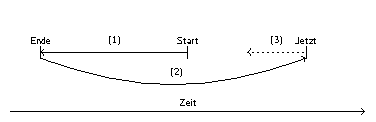
\includegraphics[width=\textwidth]{Bilder/Daemon/SearchStrategy2.pdf}
\caption{Der alternative Ansatz. Zunächst wird vom Start aus rückwärts gesucht (1). Anschließend wird zum jetzigen Zeitpunkt gesprungen (2). Von dort aus wird wieder rückwärts gesucht (3).\label{fig:search_2}}
\end{figure}

Wir haben uns für den zweiten Ansatz entschieden, da sich dieser gut mit den Einschränkungen durch Twitter verträgt und keine Phasen unterscheiden muss, wie es im ersten Ansatz der Fall ist.
Aus diesem Grund wurde auch auf die Verwendung der Streaming-API verzichtet, da der Daemon stets rückwärts sucht und nicht über gerade neu veröffentlichte Tweets sofort informiert werden muss.

\subsubsection{Details der Suchstrategie}

Auch wenn die im Daemon implementierte Suchstrategie keine unterschiedlichen Phasen besitzt, so gibt es aber doch unterschiedliche Zustände, in denen sich die Suchlogik befinden kann.
Wie bereits erwähnt, besteht die Suche aus aneinandergereihten Einzelsuchen.
Diese Einzelsuchen haben wir \emph{Iterationen} genannt.
Eine Iteration kann sich in zwei Zuständen befinden.
Hat sie noch nicht begonnen, dann wurde noch nicht nach neuen Tweets, die vor dem Zeitpunkt $t$ veröffentlicht worden sind, gesucht.
In der Iteration kann jedoch auch schon nach neuen Tweets gesucht worden sein, deren Erstelldatum vor $t$ liegt.
In diesem Fall ist die Iteration \emph{aktiv}. 

Bevor auf genaue Details der Suchlogik eingegangen werden kann, muss zunächst der Begriff der \emph{Intervalllänge} erläutert werden.
Die Intervalllänge ist ein Zeitraum, der mit einem Suchbegriff assoziiert ist.
Dieser Zeitraum bestimmt, wann erneut nach diesem Suchbegriff gesucht werden soll.
Denn nach Begriffen, die wenig Aktivität erfahren, es also über einen längeren Zeitraum nur wenige neue Tweets gibt, sollte weniger häufig gesucht werden als nach Begriffen, die eine starke Aktivität besitzen, es also permanent viele neue Tweets gibt.
Dies ist insbesondere deswegen sinnvoll, weil ein für die Suche verwendetes Twitter-Profil nur beschränkt viele Anfragen innerhalb von 15 Minuten zur Verfügung hat.
Dieser Sachverhalt wird im Abschnitt über das \textit{scheduling} weiter vertieft werden.

Zu Beginn der Suche ist die Iteration nicht aktiv.
Der Suchzeiger, der angibt, wo wir uns auf dem Zeitstrahl der Iteration befinden, steht also auf dem Zeitpunkt $t$.
In diesem Fall muss die Intervalllänge des zu bearbeitenden Suchbegriffs betrachtet werden.
Ist der Zeitraum, der zwischen der letzten Suche und $t$ liegt, kleiner als die Intervalllänge, so darf nicht nach dem Suchbegriff gesucht werden.
Wir setzen in diesem Fall $t$ neu auf den jetzigen Zeitpunkt, sodass bei einem erneuten Prüfen, ob gesucht werden soll, die Möglichkeit besteht, dass die Intervalllänge nun überschritten worden ist.
In dem Fall wird dann einmal nach Tweets gesucht, deren Erstelldatum vor $t$ liegt.
Anschließend werden für die Suche nur noch Tweets-IDs verwendet, da Twitter keine Suche nach exakten Zeitpunkten zulässt.
Dazu werden Anfragen an Twitter gestellt, die neben dem Suchbegriff auch die Tweet-ID $id$ beinhalten.
Twitter liefert dann für den Suchbegriff bis zu 100 Tweets, deren IDs kleiner als $id$ sind.
Gleichzeitig sind diese Tweets chronologisch sortiert und liegen zeitlich direkt vor dem Erstellzeitpunkt des Tweets von $id$.
Aus diesen den erhaltenen Tweets wird anschließend der älteste ausgewählt, dessen ID als neuer Suchanker dient.
So hangelt sich der Suchzeiger anhand der Tweet-IDs zeitlich rückwärts entlang, bis keine neuen Tweets mehr gefunden werden.
In dem Fall wird $t$ neu gesetzt und die aktuelle Iteration beendet.
Insbesondere wird die Intervalllänge nicht beachtet, wenn die Iteration aktiv ist.

Ein kleines Beispiel verdeutlicht diesen Ablauf:
Wir befinden uns am Anfang der Iteration, sie ist also noch nicht aktiv.
In $t$ steht der momentane Zeitpunkt und die Intervalllänge wird überschritten.
Also darf gesucht werden.
Dazu wird für einen Suchbegriff eine Anfrage an Twitter gestellt, die 100 jüngsten Tweets vor dem jetzigen Zeitpunkt zu liefern.
Twitter ermöglicht zwar keine Suche zu bestimmten Zeitpunkten, bietet jedoch die Funktionalität, die 100 jüngsten Tweets vor dem aktuellen Zeitpunkt anzufordern.
Alle Tweets werden zwischengespeichert, jedoch noch nicht in der Datenbank abgespeichert (siehe dazu Abschnitt den Abschnitt über die Architektur des Daemons).
Aus diesen Tweets wählen wir den ältesten aus und merken uns seine Tweet-ID.
In einer nächsten Anfrage liefert uns Twitter die 100 jüngsten Tweets vor dem Tweet mit der gemerkten ID.
Auch hier wählen wir wieder den ältesten aus, den wir für eine neue Anfrage nutzen können.
Dies wird so lange fortgeführt, bis keine neuen Tweets mehr gefunden werden.
Das kann zwei Ursachen haben:
Zum einen kann es sein, dass die Iteration einen viel zu langen Zeitraum überstreckt (also mehr als 6-9 Tage).
Dann liefert Twitter grundsätzlich keine Tweets mehr aus.
Also muss die Iteration beendet werden.
Zum anderen kann es aber auch sein, dass das komplette Intervall abgearbeitet wurde und wir Tweets finden, deren Erstelldatum bereits vor dem Startzeitpunkt der vorhergegangen Iteration liegen.
Diese Tweets liegen schon bereits alle in der Datenbank, weswegen die Iteration beendet werden kann.

\subsubsection{Berechnung der Intervalllänge}

Die Intervalllänge gibt an, wann zu einem Suchbegriff gesucht werden soll.
Ist noch nicht genug Zeit seit dem letzten Iterations-Startzeitpunkt vergangen, so wird noch nicht nach dem Suchbegriff gesucht.
Denn ansonsten würde sehr häufig nach Suchbegriffen gesucht werden, zu denen es keine bis nur sehr wenige, neue Tweets gibt.
So würden unnötig viele Suchanfragen gestellt und die Twitter-Profile deswegen nicht optimal ausgenutzt werden.
Es erscheint daher sinnvoll, nur dann nach Suchbegriffen zu suchen, wenn davon ausgegangen werden kann, mit einer einzigen Suchanfrage alle neuen Tweets zu finden.
Da eine Anfrage höchstens 100 Tweets liefert, muss die Anzahl der mit einer Anfrage aufzufindenden Tweets also auf 100 gesetzt sein.
Nach einem Suchbegriff, zu dem in der Stunde im Schnitt nur zwei neue Tweets veröffentlicht werden, sollte also ungefähr alle 50 Stunden gesucht werden.
Falls der Benutzer jedoch zeitiger Ergebnisse sehen möchte, kann er die Intervalllänge über die Benutzer-Priorisierung für den Suchbegriff reduzieren.
Analog können nicht so wichtige Suchbegriffe über eine negative Priorisierung eine längere Intervalllänge erhalten.

Um festzustellen, wie häufig neue Tweets zu einem Suchbegriff vorkommen, wird während der gesamten Suche der jüngste und der älteste gefundene Tweet festgehalten (nicht der jüngste und älteste einer Anfrage).
Über die über den gesamten Zeitraum zwischen ältesten und jüngsten Tweet gefundenen, neuen Tweets lassen sich die Tweets pro Minute ($TPM$) ermitteln.
Anhand der $TPM$-Zahl lässt sich der Zeitraum bestimmen, über welchem erwartungsgemäß weitere 100 neue Tweets vorhanden sein werden.
Da die Anzahl der neuen Tweets aber immer etwas schwankt und nicht konstant gleich bleibt, gibt es noch einen Korrekturwert, der mit der Intervalllänge multipliziert wird.
Der Wert wurde auf $0,9$ festgelegt.
Veranschaulicht werden dann nur 90 der 100 neuen Tweets gefunden, da nur $90\%$ des Zeitraums abgedeckt werden.
Dieser Faktor soll sicherstellen, dass leichte Abweichungen nach oben nicht eine weitere Anfrage provozieren.
Stattdessen wird der Puffer von noch 10 Tweets verwendet.
Zukünftig wird die Intervalllänge anschließend gekürzt, da nicht so viel Zeit wie durch die Intervalllänge vorgegeben ist, vergehen muss.
Falls es hingegen eine Abweichung nach unten gibt, so wird die Intervalllänge verlängert werden, da mehr Zeit verstreichen muss, bis 90 Tweets gefunden werden.

Insgesamt ergibt sich die Intervalllänge $I$ gemäß folgender Formel:

$$I = p \cdot \frac{1}{TPM} \cdot t \cdot 100,$$

wobei $p \in \{\,0,5;\,0,75;\,1;\,1,5;\,2\,\}$ der Benutzer-Priorität von positiv ($0,5$ und $0,75$) über neutral ($1$) bis negativ ($1,5$ und $2$) entspricht, $TPM$ die Tweets pro Minute sind und $t$ dem \textit{throttle factor} von $0,9$ entspricht.
Die 100 entspricht den 100 angepeilten, neuen Tweets, die es über den Zeitraum der Intervalllänge zu finden gilt.

Für den Fall, dass kein oder nur 1 Tweet gefunden wurde, wird die momentane Intervalllänge mit einem "`Außenseiter"'-Faktor multipliziert, die aktuell auf 3 gesetzt ist.
Das Eintreten dieses Falls ist unerwartet, da die Intervalllänge ja auf 90 Tweets ausgelegt war.
Aus diesem Grund wird sie verlängert, da der Suchbegriff offenbar ein unerwartetes Ereignis durchlebt haben muss, was die Intervalllänge vorher hat falsche Annahmen machen lassen.
Die Intervalllänge kann insgesamt eine Länge von sechs Tagen erreichen, nicht jedoch mehr. Dieser Wert wurde gewählt, da Twitter Tweets nur bis zu sechs Tagen in die Vergangenheit garantiert.
Dies stellt zwar nicht sicher, dass alle Tweets in dem Zeitraum der letzten Tage gefunden werden (weil vielleicht eine plötzliche, unerwartete Aktivität mit dem Suchbegriff verbunden ist), aber ein noch längeres Warten wäre sinnlos, da dann tatsächlich Tweets verloren gehen würden.
Da die Zeit für das Erneuern des \textit{rate limits} durch Twitter auf 15 Minuten festgelegt ist, sollte die Intervalllänge mindestens eine Länge von 15 Minuten besitzen.
Aus diesem Grund wird eine Intervalllänge, die laut der Formel kürzer als 15 Minuten lang ist, automatisch auf 15 Minuten festgelegt.

\subsubsection{Scheduling}
Die Anzahl der Suchanfragen innerhalb von 15 Minuten ist durch Twitter beschränkt, weswegen die Anzahl der Suchanfragen zu einer effizient zu verwaltenen Ressource wird. Aus diesem Grund wurde im Daemon ein intelligentes Verhalten zur effizienten Verwaltung der Suchbegriffe eingefügt, um möglichst nur dann eine Suche zu einem Suchbegriff zu starten, wenn dies auch sinnvoll erscheint.

Die Grundidee ist es nun, dass der Daemon immer nur dann eine Anfrage zu einem Suchbegriff startet, wenn er die 100 neuen Tweets seit dem letzten Abrufen mit einer Anfrage sammeln kann. Dies ist eine signifikante Verbesserung der Auslastung von Suchbegriffen im Vergleich zum ursprünglichen Verhalten, bei dem der Daemon zu jedem aktiven Suchbegriff immer mindestens eine Anfrage bei Verwendung eines frischen Twitter-Profils.

Um ein intelligentes Scheduling-Verhalten der Suchgriffe zu gewährleisten, werden Suchbegriffe in zwei Klassen unterteilt: \textit{short search terms} und \textit{long search terms} (auch einfach nur \textit{short terms} und \textit{long terms}).

Unter \textit{short terms} verstehen wir solche Suchbegriffe, die eine Intervalllänge \emph{länger} als die minimale, durch Twitter vorgegebene \textit{rate limit} Resetzeit besitzen, was zur Zeit 15 Minuten sind. Das bedeutet, dass zu diesem Suchbegriff idealerweise innerhalb von einer Anfrage alle neuen Tweets gefunden und gespeichert werden können, denn die Intervalllänge ist ja gerade so kalkuliert worden, dass mit einer Anfrage 100 neue Tweets gefunden werden sollten. Da davon ausgegangen wird, dass mit einer Anfrage alle neuen Tweets gefunden werden, werden diese auch nur einmal abgefragt.

Für den Fall, dass mehr als 100 Tweets vorhanden, aber nicht abgefragt worden sind, wird die Intervalllänge entsprechend korrigiert, sodass die nächste Abfrage einer neuen Iteration bereits nach kürzerer Zeit stattfindet. Da allerdings noch weitere, neue Tweets vorhanden sind, werden bei weiteren Suchen unabhängig von der Intervalllänge ab der zuletzt gefundenen Tweet-ID weitere Tweets ermittelt, da sich der Suchbegriff in einer aktiven Iteration befindet. Alle Suchvorgänge werden von einzelnen Threads, die von uns als \texttt{Minions} bezeichnet und in Abschnitt \ref{ssection:parallele-suche} ausführlich erläutert werden, durchgeführt.

Gibt es beispielsweise einen \textit{short term}, nach dem gesucht werden soll, so wird dieser \textit{short term} einem neuen gestarteten \texttt{Minion} zugewiesen.
Dieser sucht dann ein einziges Mal nach Tweets zu diesem Suchbegriff.
Unabhängig davon, wie viele Tweets gefunden wurden, wird die Intervalllänge zu diesem Suchbegriff angepasst.
Nachdem sich der \texttt{Minion} beendet hat, weil er entweder sein \textit{rate limit} aufgebraucht hat oder alle Iterationen zu seinen zugewiesenen Suchbegriffen beendet hat, wird der \textit{short term} erneut einem weiteren \texttt{Minion} zugeordnet.
Dieser \texttt{Minion} sucht auf jeden Fall noch einmal nach Tweets zu diesem \textit{short term}, da der \textit{short term} sich momentan in einer aktiven Iteration befindet.
Jetzt gibt es allerdings zwei mögliche Situationen.
Zum einen kann es vorkommen, dass der \texttt{Minion} keine neuen Tweets mehr zu dem Suchbegriff findet.
In dem Fall ist die Iteration beendet.
Findet er hingegen noch neue Tweets, so darf die Iteration noch nicht beendet werden.
Dann werden weitere \texttt{Minions} zu dem \textit{short term} nach neuen Tweets suchen, bis die Iteration beendet werden kann.

Im oben genannten Szenario kann es durchaus passieren, dass ein \textit{short terms} während einer Iteration zu einem \textit{long term} wird, nämlich genau dann, wenn die Intervalllänge auf 15 Minuten korrigiert wird. Dies ist auch wünschenswert, da der \textit{short term} offenbar eine Veränderung in der Aktivität durchläuft und somit nicht mehr als \textit{short term} bezeichnet werden sollte.
Alle \textit{short terms} werden vor den \textit{long terms} abgearbeitet, da ansonsten die \textit{long terms} alle Anfragen des Twitter-Profils aufbrauchen könnten und somit nicht mehr nach den \textit{short terms} gesucht werden könnte. 

Neben den zuvor genannten \textit{short terms} gibt es noch \textit{long terms}.
Unter \textit{long terms} verstehen wir solche Suchbegriffe, die eine Intervalllänge von genau 15 Minuten besitzen.
Das bedeutet, dass angenommen wird, dass zu diesem Suchbegriff innerhalb von 15 Minuten mindestens 100 neue Tweets auftreten.
Aus Erfahrung kann jedoch davon ausgegangen werden, dass es deutlich mehr als 100 neue Tweets sind.
Aus diesem Grund werden für die nach Abarbeiten der \textit{short terms} verbliebenen \textit{long terms} auch alle restlichen Anfragen reserviert.

Ein \textit{long term} wird, anders als ein \textit{short term}, nicht nur einmal von einem \texttt{Minion} abgearbeitet, sondern so lange bis alle Anfragen aufgebraucht sind oder die Iteration zu dem Suchbegriff beendet werden kann. So ist gewährleistet, dass \textit{long terms} der großen Datenmenge an Tweets auch nachkommen. Die \textit{long terms} werden gemäß einer \textit{round robin} Strategie durchgegangen, sodass jeder Suchbegriff annähernd gleich viele Anfragen erhält.

Der Name \textit{long term} rührt daher, dass nach diesen Suchbegriffe lange gesucht werden muss, während \textit{short terms} nur eine kurze Suchzeit besitzen. Eine mögliche alternative Interpretation der Namen bezüglich der Dauer der Intervalllänge wurde nicht gewählt.

Die Aufgabe des Daemons ist es, permanent Daten zu allen aktiven Suchbegriffen zu sammeln.
Dabei ist es durchaus sinnvoll, jüngere Suchbegriffe ein wenig zu priorisieren, da zu diesen Suchbegriffen möglichst schnell ein repräsentativer Datenbestand aufgebaut werden soll.
Gleichzeitig besitzen ältere Suchbegriffe bereits einen relativ zum Suchbegriff ausreichend großen Datenbestand.

Aus diesem Grund werden sowohl die Liste der \textit{short terms} als auch \textit{long terms} zeitlich sortiert, sodass am Anfang der Listen der jüngste Suchbegriff steht. Am Beispiel der \textit{long terms} werden wir sehen, weswegen diese Sortierung eine leichte Priorisierung bewirkt.

Wir stellen uns das folgende Szenario vor.
Es sind fünf \textit{long terms} vorhanden, wovon ein Suchbegriff jung und die restlichen Suchbegriffe alt sind.
Zusätzlich stehen nur noch zwölf Anfragen zur Verfügung.
Die Liste wird nun zeitlich sortiert, sodass der junge Suchbegriff ganz am Anfang steht.
Er bekommt die erste Anfrage.
Anschließend sind die älteren Suchbegriffe an der Reihe.
Jetzt hat jeder Suchbegriff einmal eine Anfrage stellen dürfen und es sind noch sieben Anfragen verfügbar.
Bei einem weiteren Durchlauf erhält ebenfalls wieder jeder Suchbegriff eine Anfrage.
Jetzt stehen jedoch nur noch zwei Anfragen zur Verfügung, das heißt nicht jeder Suchbegriff kann eine Anfrage stellen.
Es ist daher sinnvoll, die verbliebenen Anfragen auf die Suchbegriffe zu verteilen, die es noch am Nötigsten haben, ihren Datenbestand zu erweitern.
Dies ist bei jüngeren Suchbegriffen der Fall.
Aus diesem Grund werden die zwei übrig gebliebenen Anfragen auf die ersten beiden Suchbegriffe verteilt.
Darunter ist auch der junge Suchbegriff.
Jetzt hat dieser Suchbegriff eine Anfrage mehr als fast alle anderen Suchbegriffe erhalten und wurde somit gemäß seines Alters priorisiert. 

Die Priorisierung durch die zeitliche Sortierung ist jedoch nur eine Art, wie jüngere Suchbegriffe bevorzugt werden.
Eine viel stärkere Priorisierung ergibt sich durch so genannte virtuelle Kopien von zu priorisierenden Suchbegriffen.
Gemäß der Einteilung eines Suchbegriffs in jung (weniger als einen Tag alt), etwas älter (weniger als eine Woche, aber mindestens einen Tag alt) und alt (mehr als eine Woche alt) werden zu den Suchbegriffen unterschiedlich viele virtuelle Kopien erstellt und, ebenfalls zeitlich sortiert, an das Ende der Liste der von einem \texttt{Minion} abzuarbeitenden Suchbegriffe angehängt.
Diese virtuellen Kopien werden wie ganz normale \textit{long terms} behandelt, sodass dem zugrundeliegenden Suchbegriff insgesamt mehr Anfragen zukommen.
Für \textit{short terms} gibt es diese Priorisierung nicht, da ja davon ausgegangen wird, dass mit einer Anfrage bereits alle neuen Tweets gefunden wurden.

Ein Beispiel soll diesen Sachverhalt verdeutlichen. Wir haben wieder fünf Suchbegriffe gegeben, wobei einer davon jung, ein anderer etwas älter und die restlichen Suchbegriffe alt sind.
Wenn wir annehmen, dass junge Suchbegriffe insgesamt pro \textit{round robin} Runde $a$ Anfragen, etwas ältere Suchbegriffe insgesamt $b$ Anfragen und alte Suchbegriffe insgesamt $c$ Anfragen erhalten sollen, wobei $a \geq b \geq c$ gilt, sähe die Liste nach Priorisierung durch virtuelle Kopien wie in Abbildung \ref{figure:daemon_virt_copies} dargestellt aus.

\begin{figure}
\centering
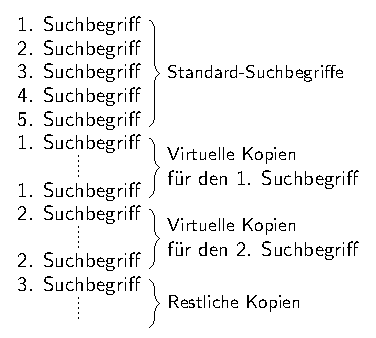
\includegraphics[width=0.4\textwidth]{Bilder/Daemon/VirtualCopies.pdf}
\caption{Die Aufteilung der virtuellen Kopien zu den einzelnen Suchbegriffen. Diese Liste wird anschließend an einen \texttt{Minion} zur Abarbeitung übergeben. \label{figure:daemon_virt_copies}}
\end{figure}

Wie der Abbildung zu entnehmen ist, besitzen junge Suchbegriffe insgesamt $(a - c)$ Anfragen mehr als alte und $(a - b)$ Anfragen mehr als etwas ältere Suchbegriffe.
Zudem haben etwas ältere Suchbegriffe $(b - c)$ Anfragen mehr zur Verfügung als alte Suchbegriffe. Durch diese Priorisierung anhand von virtuellen Kopien wird der Datenbestand für jüngere Begriffe schneller aufgefüllt als bei älteren. 

Momentan ist die Aufteilung für virtuelle Kopien wie folgt:
\begin{itemize}
\item Der Suchbegriff ist weniger als einen Tag alt: 2 weitere virtuelle Kopien
\item Der Suchbegriff ist weniger als eine Woche, aber mindestens einen Tag alt: 1 weitere virtuelle Kopie
\item Der Suchbegriff ist älter als eine Woche: keine weiteren virtuellen Kopien
\end{itemize}

Die Suchstrategie des Daemons zu einem Suchbegriff wird also beeinflusst durch
\begin{itemize}
\item die Intervalllänge für des Suchbegriffes,
\item die durch den Benutzer vorgegebene Priorität zu dem Suchbegriff,
\item das Aktivitätsverhalten des Suchbegriffs, das den Suchbegriff als \textit{short} oder \textit{long term} klassifiziert und
\item das Alter des Suchbegriffs, was zu einer unterschiedlichen Anzahl an virtuellen Kopien und somit zu einer unterschiedlichen Anzahl von Anfragen zum Suchbegriff führt. 
\end{itemize}

\subsection{Parallele Suche} % Jens
\label{ssection:parallele-suche}
\subsubsection{Motivation}
Nachdem der Daemon in der Lage ist mit einer gewissen Intelligenz Tweets zu suchen, könnte man annehmen der Daemon sei fertig.
Für Untersuchungen im kleineren Umfang ist das prinzipiell auch korrekt, uns war die Menge der gefundenen Tweets aber nicht hoch genug.
Wie sich aus den Beschränkungen der Twitter-API, die in Abschnitt \ref{sssection:twitter-api} beschrieben wurden, ergibt, kann der Daemon mit einem Profil maximal 18.000 Tweets in 15 Minuten sammeln.
Das ist vergleichsweise wenig, besonders wenn die Anzahl der Suchbegriffe steigt und auch sehr aktive Suchbegriffe, das heißt Suchbegriffe zu denen es aufgrund gesteigerten Interesses sehr viele Tweets gibt, dabei sind.
Ein Beispiel für einen sehr aktiven Suchbegriff war \textit{walker}.
Mit diesem \textit{search term} konnte man sehr viele Tweets zum Tod von Schauspieler Paul Walker, am 30. November 2013 finden, insgesamt ca. 11 Millionen innerhalb weniger Tage.
Diese Zahlen berichtete zumindest Topsy\footnote{\url{www.topsy.com}}, sie sind aber leider nicht mehr abrufbar, allerdings findet sich im November/Dezember 2013 auch bei Google Trends \cite{GoogleTrendsWalker14} ein entsprechender Ausschlag im Interesse.
Die Anzahl Tweets war zu groß, als dass unser Daemon sie alle hätte finden können.
Das liegt daran, dass der Daemon, wie in Abschnitt Twitter-API \ref{sssection:twitter-api} beschrieben, maximal 18.000 Tweets in 15 Minuten abrufen kann und wir über die Suche maximal 6-9 Tage zurückliegende Tweets finden können.
Da wir noch mehr als diesen einen Suchbegriff bearbeiten, ist es in dem zur Verfügung stehenden Zeitfenster von 6-9 Tagen also nicht möglich alle Tweets zu diesem Thema zu erfassen.
Deswegen wurde als nächstes Ziel entschieden, den Durchsatz zu erhöhen.
Der für uns nächstliegendste Ansatz war der Einsatz mehrerer Profile, immerhin erlaubt jedes weitere Profil den Abruf von bis zu 18.000 weiteren Tweets.
Um mehrere Profile optimal auszunutzen, müssen sie  parallel genutzt werden.
Das erlaubt sowohl die parallele Suche nach verschiedenen Suchbegriffen, als auch nacheinander mit verschiedenen Profilen nach einem Suchbegriff zu suchen.
Da die Suche selbst auch einige Zeit in Anspruch nimmt, kann dies nicht beliebig gesteigert werden, erlaubt aber doch eine gewisse Skalierung.
Gerade auch im Bezug auf eine steigende Zahl von Suchbegriffen erlaubt dies eine höhere Anzahl von gefundenen Tweets.

\subsubsection{Architektur} % Master - Worker - Aufbau - Minions 
Das Parallelisieren erfolgt in einer klassischen Master-Worker-Architektur, bei der ein Master Aufgaben an mehrere Worker verteilt und ihre Ergebnisse sammelt.
Dies erfordert eine Überarbeitung unserer bestehenden Architektur.
Unser Master heißt auch \texttt{Master}, während wir unsere Worker \texttt{Minions} genannt haben.
Außerdem soll der Daemon jetzt dauerhaft laufen und nicht wie vorher nur alle 15 Minuten durch einen \textit{cronjob} gestartet werden.
Dabei ist der \texttt{Master} für die Verwaltung der Profile und die Aufteilung der Suchbegriffe auf die \texttt{Minions} zuständig, während die \texttt{Minions} selbst nur die Tweets von Twitter abrufen und speichern sollen.

\subsubsection{Architektur: Master}% Der Master
Die Suchbegriffe holt sich der \texttt{Master} aus der Datenbank, nachdem er sie in \textit{short} und \textit{long terms} eingeteilt hat (siehe Suchstrategie \ref{ssection:Suchstrategie}), erhält der erste \texttt{Minion} mit einem gültigem Profil, d.\,h. mit einem Profil das noch freie Suchanfragen hat, eine bestimmte Anzahl davon und beginnt mit der Suche.
Wie der \texttt{Master} Suchbegriffe aus der Datenbank abruft und an die \texttt{Minions} verteilt ist in Grafik \ref{img:daemonarchitektur1} dargestellt.
%Wenn der \texttt{Master} gestartet wird und sowohl aktive Suchbegriffe als auch gültige Profile, d.\,h. Profile mit offenen Anfragen, hat, startet er einen \texttt{Minion} und teilt ihm Suchbegriffe zu.
Dabei merkt der \texttt{Master} sich, welche Suchbegriffe er schon verteilt hat, und registriert auch, wenn ein \texttt{Minion} mit seiner Arbeit fertig ist, seine Suchbegriffe also wieder frei werden.
Ursprünglich ging der \texttt{Master} davon aus, dass alle Profile gültig sind, wenn er gestartet wird. Falls dem nicht so war konnte das dazu führen, dass der \texttt{Master} in einer Art Endlos-Schleife lief, dies aber nur temporär.
%TODO eine temporäre Endlos-Schleife ??
In der Schleife hat der \texttt{Master} immer wieder einen \texttt{Minion} erzeugt. Dieser hat sich aber sofort wieder beendet, weil er keine Anfragen mehr frei hatte.
Da der \texttt{Master} die Profile der Reihe nach durchgeht, hängt er so lange in der Schleife bis das Profil wieder gültig wird.
Um diese Problematik zu beheben, wurde die Abfrage der noch freien Anfragen von den \texttt{Minions} in den \texttt{Master} verlagert.
Dadurch weiß der \texttt{Master} immer, ob ein Profil gültig ist.
Wenn der \texttt{Master} keine gültigen Profile oder keine aktiven Suchbegriffe mehr hat, schläft er für einen gewissen, einstellbaren Zeitraum, bevor er erneut prüft, ob es aktive Suchbegriffe und gültige Profile gibt.

\begin{figure}[ht]
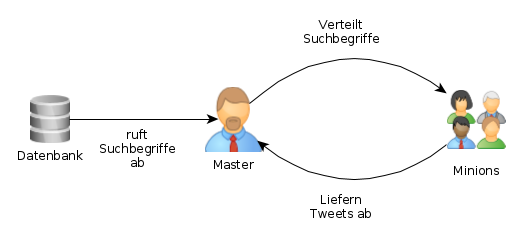
\includegraphics[width=\textwidth]{Bilder/Daemon/DaemonArchitektur1.png}
\caption{Der \texttt{Master} holt Suchbegriffe aus der Datenbank und verteilt sie an die \texttt{Minions}.}
\label{img:daemonarchitektur1}
\end{figure}

\subsubsection{Architektur: Minions} % Die Minions: wie arbeiten sie - speichern selber tweets -> überleitung treasurer
Die Hauptaufgabe der \texttt{Minions} ist das Suchen und Speichern von Tweets.
Große Teile dieser Aufgaben konnten direkt aus dem Code der vorherigen \texttt{single-threaded} Anwendung übernommen werden.
Die Suchbegriffe, die jeder \texttt{Minion} bearbeitet, erhält er dabei direkt vom \texttt{Master}, sodass sich die \texttt{Minions} nicht darum kümmern müssen, welche Begriffe aktiv und noch nicht von anderen \texttt{Minions} belegt sind.
Der \texttt{Master} erhält die Suchbegriffe dabei über den \texttt{Transactor}, der Schnittstelle zur Datenbank, direkt aus der Datenbank.
Sobald ein \texttt{Minion} alle seiner Anfragen aufgebraucht hat, hat er sie über den \texttt{Transactor} in der Datenbank gespeichert.
Es musste sichergestellt werden, dass nicht mehrere \texttt{Minions}, oder ein \texttt{Minion} und der \texttt{Master} gleichzeitig oder in der falschen Reihenfolge auf den gleichen Suchbegriff zugreifen.
Schlimmstenfalls könnte es sonst passieren, dass zwei \texttt{Minions} in der falschen Reihenfolge versuchen, denselben Suchbegriff zu updaten und das Programm dabei abstürzt.
Dies würde zu inkonsistenten Werten bei dem Suchbegriff und damit verlorenen Tweets, d.\,h. Tweets die wir zwar finden könnten, aber nicht erfasst haben, führen.
Auch würden so Anfragen verschwendet, wenn der \texttt{Master} einen neuen \texttt{Minion} zu einem Suchbegriff gestartet hat, der mit genau den gleichen Parametern schon vom vorherigen \texttt{Minion} bearbeitet wurde, diese Werte aber noch nicht in der Datenbank aktualisieren konnte.
Ebenfalls stellte sich schnell heraus, dass die Datenbank-Performance erheblich darunter gelitten hat, wenn zwei \texttt{Minions} gleichzeitig ihre Tweets gespeichert haben.


\subsubsection{Architektur: Treasurer}% Tweets Zentral speichern / Treasurer #1
Um das Problem zu lösen, entschieden wir uns dafür, das Speichern der Tweets und das Aktualisieren der Suchbegriffe an eine zentrale Stelle auszulagern.
Das geschieht, indem die \texttt{Minions} die Tweets, die sie erhalten haben, zusammen mit den entsprechenden und aktualisierten Suchbegriffen beim \texttt{Master} abliefern.
Der \texttt{Master} aktualisiert daraufhin sein lokales \texttt{SearchTerm}-Objekt und speichert die erhaltenen Tweets zwischen.
Dabei stellen alle Tweets inklusive des dazugehörigen Suchbegriffs und seiner Parameter ein \texttt{Package} dar.
Alle \texttt{Packages} werden in einem Beutel gesammelt und nach dem Datum des letztens Abrufs sortiert.
Der Beutel ist dabei, ähnlich wie die \texttt{Treasury} ein virtuelles Konstrukt, in diesem Fall für einen Zwischenspeicher, um \texttt{Packages} zu sammeln.
So stellen wir sicher, dass die \texttt{Packages} in der richtigen Reihenfolge in der Datenbank gespeichert werden.
Falls wir das nicht täten, könnten wir Tweets verlieren.
Wenn der \texttt{Master} von der Datenbank neue Suchbegriffe erhält, vergleicht er sie mit seinen lokalen Objekten.
Solange seine lokalen Objekte neuere Werte haben als die Werte, die die Datenbank liefert, werden die lokalen verwendet.
Ausschlaggebendes Kriterium dafür, wie aktuell ein Suchbegriff ist, ist der Zeitpunkt der letzten Suche.

\begin{figure}[ht]
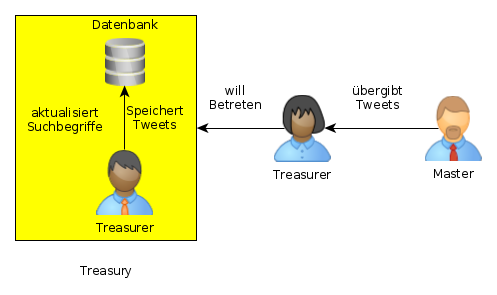
\includegraphics[width=\textwidth]{Bilder/Daemon/DaemonArchitektur2.png}
\caption{Der \texttt{Master} übergibt die gesammelten Tweets einem \texttt{Treasurer}. Ein weiterer \texttt{Treasurer} speichert Tweets in die Datenbank.}
\label{img:daemonarchitektur2}
\end{figure}

%Tweets Zentral speichern / Treasurer #2
Der \texttt{Master} soll nicht selbst die Tweets speichern, da er zum einen weiterhin neue Tweets der \texttt{Minions} entgegennehmen, zum anderen auch die Suchbegriffe verteilen muss.
Um dies zu umgehen, wurde ein neuer \texttt{Worker} erschaffen, dessen einzige Aufgabe das Speichern von Tweets ist.
Wir haben ihn \texttt{Treasurer} genannt, analog dazu gibt es auch eine \texttt{Treasury}, eine Schatzkammer.
Die \texttt{Treasury} ist dabei ein virtuelles Konstrukt, das den Zugang zur Datenbank bildlich darstellt.
Der \texttt{Master} wartet entweder, bis er mindestens eine gewisse Anzahl von Tweets in seinem Beutel gesammelt hat, oder bis eine einstellbare Zeit nach dem Ende des letzten \texttt{Treasurer} vergangen ist, bis er einen neuen \texttt{Treasurer} erzeugt.
Es kann dabei durchaus mehrere \texttt{Treasurer} gleichzeitig geben, wenn sehr viele Tweets in kurzer Zeit gefunden werden, oder die alten \texttt{Treasurer} noch nicht mit ihrer Arbeit fertig sind, wenn ein neuer erzeugt wird.
Der \texttt{Treasurer} erhält eine Kopie des Beutels vom \texttt{Master} und dieser leert anschließend seinen Beutel.
Nun versucht der \texttt{Treasurer} die \texttt{Treasury} zu betreten.
Wie der Master die gesammelten Tweets an einen \texttt{Treasurer} übergibt, während ein weiterer \texttt{Treasurer} Tweets in der Datenbank speichert, ist in Grafik \ref{img:daemonarchitektur2} dargestellt.
Die \texttt{Treasury} ist dabei als Mutex realisiert und stellt somit auch eine Warteschlange für die \texttt{Treasurer} da.
Versucht ein \texttt{Treasurer} die \texttt{Treasury} zu betreten, heißt das, dass er versucht das Mutex zu erlangen.
Gelingt ihm das Betreten der \texttt{Treasury}, also das Erlangen des Mutex, speichert er alle Tweets aus seinem Beutel in der Datenbank, genau wie es der alte Daemon vorher getan hat.
Außerdem aktualisiert er die \texttt{SearchTerms} in der Datenbank, allerdings erst, nachdem er die zu dem Suchbegriff gehörenden Tweets gespeichert hat.
Falls der Daemon abstürzt oder beendet wird, bevor der Suchbegriff aktualisiert wurde, sind die Tweets trotzdem vorhanden und werden schlimmstenfalls erneut gefunden.
Würde aber erst der \texttt{SearchTerm} aktualisiert und danach erst die Tweets gespeichert, wären alle Tweets verloren, die nicht mehr gespeichert wurden.
Das liegt daran, dass der Daemon aufgrund seiner Suchstrategie davon ausgeht, dass die Tweets schon gespeichert sind.
Anschließend informiert er gegebenenfalls andere wartende \texttt{Treasurer} über das Ende seiner Arbeit und beendet sich.
Sollte die \texttt{Treasury} belegt sein, schläft ein \texttt{Treasurer} und wartet auf eine Benachrichtigung durch den die \texttt{Treasury} belegenden \texttt{Treasurer}.
In der letzten Scrum-Iteration des Projektseminars wurde die Art, wie der \texttt{Treasurer} die Tweets in der Datenbank speichert, angepasst.
Waren es zuerst jeweils einzelne Tweets, die gespeichert wurden, wurde das System auf \textit{batch inserts} umgestellt.
Dabei fügt der \texttt{Treasurer} erst eine bestimmte Anzahl von Tweets zu einem \textit{batch} zusammen und speichert dann alle Tweets einer \textit{batch} auf einmal.
Dies brachte teilweise erhebliche Geschwindigkeitsvorteile, auch abhängig von der Größe der \textit{batch}.

\subsubsection{Multi-Threading}
Die parallele Suche an sich wurde mit einem klassischen Master-Worker Modell mit Multi-Threading umgesetzt.
Der \texttt{Master} hat dabei hauptsächlich die verwaltende Tätigkeit, wie oben beschrieben.
Generell ist sowohl der \texttt{Master} als auch jeder \texttt{Minion} und \texttt{Treasurer} ein eigener Thread.
Ein Abstürzen eines einzelnen Threads sollte, solange es sich nicht um den \texttt{Master} handelt, nicht das ganze Programm abstürzen lassen.
Es gab aber an einigen Stellen Schwierigkeiten mit dem Multi-Threading Ansatz.
So müssen die einzelnen Worker mit dem \texttt{Master} interagieren und z.\,B. melden, wenn sie mit ihrer Arbeit fertig sind.
Auch gibt es mehrere Stellen, an denen mehrere Threads um die gleiche Ressource kämpfen, wo es Probleme mit Deadlocks gab.
Ein klassisches Problem war dabei, dass in der \texttt{Treasury} der Mutex nicht überall in der gleichen Reihenfolge erlangt wurde, dies konnte zu Deadlocks führen.
Die Lösung war die Reihenfolge, in der die Mutexe erlangt werden, überall zu vereinheitlichen.
Ein weiteres Problem konnte auftreten, wenn der \texttt{Master} keine freien Suchbegriffe hatte.
Dabei hat er eine \texttt{if}-Abfrage abgebrochen, in dessen Rahmen ein Mutex erlangt wurde, ohne es frei zu geben.
Da die \texttt{Minions} aber denselben Mutex benötigten, um ihre Tweets und Suchbegriffe abzugeben, kam es zu einem Deadlock. Das Finden dieses Fehlers war sehr aufwändig.
Die Lösung, dass der \texttt{Master}, bevor er die Schleife abbricht, noch den Mutex freigibt, ist dagegen recht trivial.
Das Multi-Threading erforderte auch die Einführung der schon oben erwähnten \texttt{Packages}.
Alle Tweets, die ein \texttt{Minion} findet, sind mit dem Suchbegriff, zu dem sie gefunden wurden, sowie den zugehörigen Metadaten zum Zeitpunkt der Suche verknüpft.
Wenn nun nacheinander mehrere \texttt{Minions} denselben Suchbegriff bearbeiten, gäbe es mehrere Tweets, die alle zum selben Suchbegriff gehören, aber mit unterschiedlichen Metadaten assoziiert sind.
Es war also nicht möglich alle Tweets zu einem Suchbegriff im Beutel des \texttt{Master} zu sammeln.
Stattdessen wurden \texttt{Packages} eingeführt.
Jedes \texttt{Package} stellt dabei eine Sammlung der Tweets mit dem assoziierten Suchbegriff eines Suchdurchlaufs dar.
Die einzelnen \texttt{Packages} werden dann nach dem Zeitpunkt der Suche chronologisch sortiert und auch in derselben Reihenfolge abgespeichert.
So wird verhindert, dass im Falle eines Absturzes des Programms Tweets verloren gehen, wenn sie weder gespeichert sind, noch erneut gesucht werden.

 % torsten
\subsection{Zeitnahe Ergebnisse}
\label{ssection:ZeitnaheErgebnisse}
Bislang musste der Benutzer im schlimmsten Fall bis zu 15 Minuten auf Ergebnisse warten, wenn er einen neuen Suchbegriff eingegeben hat.
Denn hatten alle zur Suche verwendeten Profile kurz bevor der Benutzer die Suche zu einem neuen Suchbegriff startete ihr \textit{rate limit} ausgeschöpft, so musste er warten, bis wieder ein Profil frei wurde.
Dies konnte aber wie bereits erwähnt dann bis zu 15 Minuten dauern.
Das war jedoch nicht besonders benutzerfreundlich und wurde daher als Problem angesehen, das es zu beheben galt.

\subsubsection{Motivation}

Es wäre daher besser, wenn der Benutzer einen neuen Suchbegriff eingibt und anschließend nach möglichst kurzer Zeit, maximal nach 20 bis 30 Sekunden, die ersten Ergebnisse seiner Suchanfrage angezeigt bekommt.
Die Anzahl der Ergebnisse muss noch nicht sehr hoch sein; vielmehr genügt es dem Benutzer, wenn er zumindest einen kleinen Datensatz als Grundlage zum Analysieren besitzt.
So kann er sich bereits sehr zeitnah einen ersten Überblick über den Suchbegriff verschaffen.
Zu einem späteren Zeitpunkt haben sich dann wesentlich mehr Daten zum Suchbegriff gefunden, mit denen der Benutzer dann intensiver arbeiten kann.

\subsubsection{Konzept}

Es stellt sich nun die Frage, wie erreicht werden kann, dass bereits sehr zeitnah zur Suchanfrage die ersten Daten präsentiert werden können.
Um das oben geschilderte Problem der aufgebrauchten Twitter-Profile zu umgehen, führen wir ein weiteres Profil ein, das nur genutzt wird, wenn ein neuer Suchbegriff in der Datenbank gefunden wird.
So ist sichergestellt, dass es immer ein Profil gibt, das nach Tweets zum neuen Suchbegriff suchen kann.
Des Weiteren darf dieses gesonderte Profil jedoch nicht sofort für einen neuen Suchbegriff das \textit{rate limit} vollständig aufbrauchen, weswegen die Anzahl der Anfragen an Twitter durch den Daemon begrenzt wird.
Wäre die Anzahl der Anfragen nicht begrenzt, so stünden für einen weiteren, neuen Suchbegriff keine Anfragen mehr zur Verfügung und der Benutzer müsste wieder 15 Minuten warten.
Die maximal zulässige Anzahl an Anfragen für das gesonderte Profil lässt sich beliebig einstellen; ein Grenzwert von 10 hat sich jedoch als akzeptabel herausgestellt.
In diesem Fall verbraucht das Profil also lediglich 10 der 180 Anfragen, weswegen noch 170 Anfragen zur Verfügung stehen.
Es kann also innerhalb von 15 Minuten nach höchstens 18 neuen Suchbegriffen gesucht werden.
Da es jedoch unwahrscheinlich ist, dass in diesem kurzen Zeitraum tatsächlich so viele neue Suchbegriffe hinzukommen, ist diese Limitierung als nicht-kritisch anzusehen.

Mit 10 Anfragen lassen sich bis zu 1000 Tweets zu einem neuen Suchbegriff finden, was eine akzeptable erste Datenbasis schafft.
Möchte man mehr Tweets finden, so muss der Grenzwert der Anfragen an Twitter hochgestellt werden.
In diesem Fall können jedoch nicht 18 neue Suchbegriffe innerhalb von 15 Minuten gefunden werden, sondern es sind weniger.
Ein Verringern des Grenzwertes liefert zwar weniger Tweets, doch kann der Benutzer dann mehr als 18 neue Suchbegriffe innerhalb der 15 Minuten eingeben.

Es sollte jedoch bedacht werden, dass ein geringer Grenzwert mit wenigen Anfragen auch weniger Zeit für die Suche nach Tweets benötigt als ein höherer Grenzwert mit mehr Anfragen.

\begin{figure}[h!]
\centering

\begin{subfigure}[t]{0.5\textwidth}
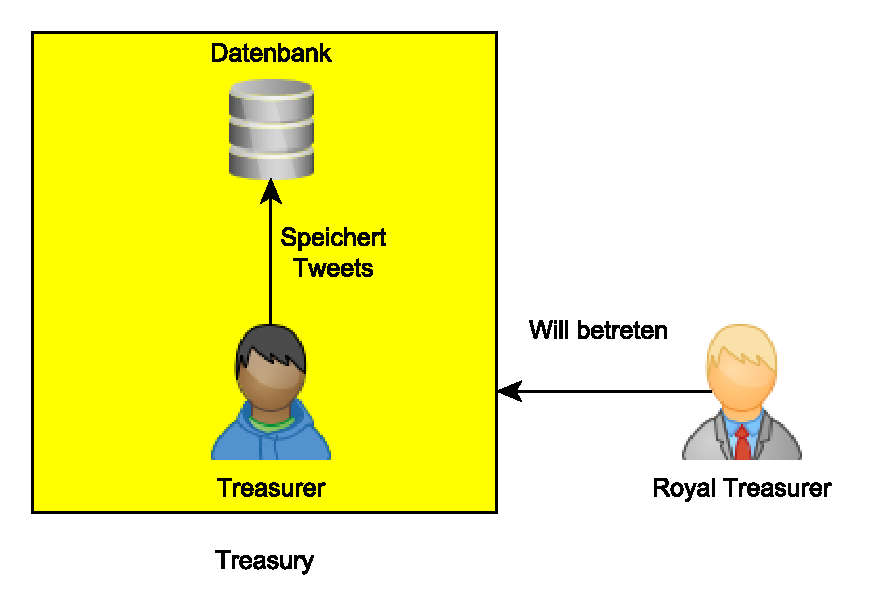
\includegraphics[width=\textwidth]{Bilder/Daemon/RoyalTreasurer1.pdf}
\caption{Ein \texttt{Royal Treasurer} will die \texttt{Treasury} betreten.}
\label{fig:royal_treasurer1}
\end{subfigure}
~
\begin{subfigure}[t]{0.3\textwidth}
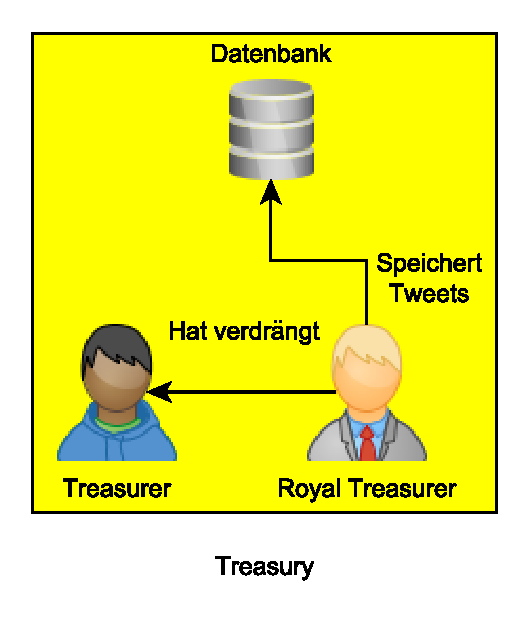
\includegraphics[width=\textwidth]{Bilder/Daemon/RoyalTreasurer2.pdf}
\caption{Der \texttt{Royal Treasurer} verdrängt den \texttt{Treasurer}.}
\label{fig:royal_treasurer2}
\end{subfigure}

\begin{subfigure}[t]{0.3\textwidth}
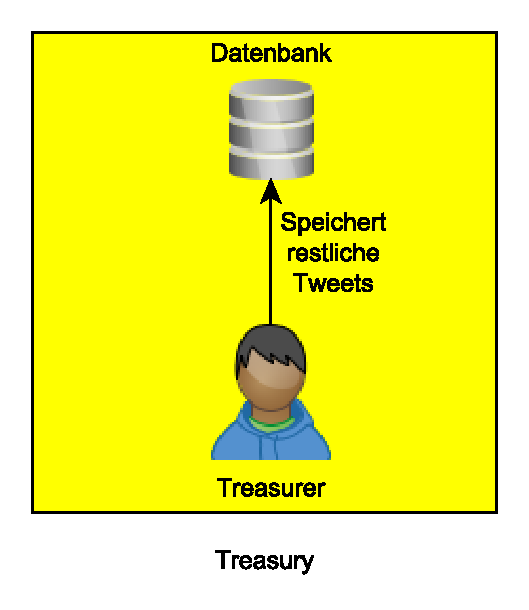
\includegraphics[width=\textwidth]{Bilder/Daemon/RoyalTreasurer3.pdf}
\caption{Der verdrängte \texttt{Treasurer} setzt seine Arbeit fort.}
\label{fig:royal_treasurer3}
\end{subfigure}
\end{figure}

Das besondere Profil alleine hilft allerdings noch nicht dabei, dass der Benutzer auch zeitnah die gefundenen Tweets angezeigt bekommt.
Bislang ist lediglich sichergestellt, dass der Daemon auf jeden Fall nach einem neuen Suchbegriff suchen kann.
Bis die Ergebnisse allerdings dem Benutzer auch tatsächlich präsentiert werden können, kann jedoch ebenfalls einige Zeit vergehen, da die Tweets noch nicht in der Datenbank gespeichert wurden.
Stattdessen werden sie zunächst im Beutel des \texttt{Masters} hinterlegt, welcher jedoch nicht zwingend umgehend durch einen \texttt{Treasurer} geleert werden muss.
Da der \texttt{Treasurer} eine vorgegebene Zeit wartet, bis er den Beutel des \texttt{Masters} leert, oder er den Beutel leert, falls die festgelegte Zahl der Tweets im Beutel überschritten wird, kann es teilweise sehr lange dauern, bis die neuen Tweets in die Datenbank geschrieben wurden.
Der Benutzer musste also weiterhin lange auf die ersten Ergebnisse warten.

Um das Problem zu umgehen, wird ein weiterer Beutel eingeführt, der ausschließlich für die zeitnahen Tweets genutzt wird.
Wurde dieser Beutel befüllt, wird er -- unabhängig davon, wann er zuletzt befüllt worden ist oder wie voll er ist -- sofort von einem \texttt{Treasurer} geleert, damit die Tweets auch sofort in die Datenbank geschrieben werden können.
Somit wurde die Wartezeit bis zur Leerung des Beutels eliminiert.
Dies hilft allerdings immer noch nicht zwingend.
Denn es kann durchaus vorkommen, dass bereits ein anderer \texttt{Treasurer} in der \texttt{Treasury} aktiv ist und unser wichtigerer \texttt{Treasurer} warten muss, was bedeutet, dass auch der Benutzer warten muss.
Aus diesem Grund erhält der \texttt{Treasurer}, der den besonderen Beutel leert, eine höhere Priorität gegenüber anderen \texttt{Treasurern}.
Um die höhe Priorität anzudeuten, wird dieser \texttt{Treasurer} deswegen \texttt{Royal Treasurer} genannt.
Betritt dieser nun die \texttt{Treasury}, verdrängt er einen möglicherweise aktiven \texttt{Treasurer} und kann somit seine Tweets sofort abspeichern.
Ist er mit dem Abspeichern fertig, so weckt er den verdrängten Treasurer wieder auf, sodass dieser seine Arbeit an dem Punkt fortsetzen kann, an dem er unterbrochen wurde.
Die Abbildungen \ref{fig:royal_treasurer1}, \ref{fig:royal_treasurer2} und \ref{fig:royal_treasurer3} illustrieren diese Situation.

Es kann vorkommen, dass es zeitweise mehrere \texttt{Royal Treasurer} gibt, nämlich genau dann, wenn mehrere Suchbegriffe zeitnah neu eingegeben werden.
Tritt diese Situation ein, so werden die \texttt{Royal Treasurer} sequentiell in der Reihenfolge, in der sie die \texttt{Treasury} betreten, aktiv.
Ein möglicherweise zuvor verdrängter \texttt{Treasurer} muss dann die gesamte Zeit lang warten, bis alle Royal \texttt{Treasurer} fertig sind.

\subsubsection{Implementierung}

Das besondere Profil wird von einem besonderen \texttt{Minion} genutzt, der darauf achtet, dass der zuvor gesetzte Grenzwert von beispielsweise zehn Anfragen auch beachtet wird.
Die anderen \texttt{Minions} suchen nämlich so lange zu Suchbegriffen, bis ihr \textit{rate limit} aufgebraucht ist.
Der besondere \texttt{Minion} wird von uns \texttt{Limited Minion} genannt, da er nur eine begrenzte (engl.: \textit{limited}) Anzahl an Anfragen an Twitter stellt.
Der \texttt{Limited Minion} teilt, nachdem er seine Suche abgeschlossen hat, dem \texttt{Master} über eine gesonderte Nachricht mit, dass er fertig ist.
Aufgrund dieser gesonderten Nachricht weiß der \texttt{Master} anschließend, dass es sich um den \texttt{Limited Minion} handelt, weswegen der \texttt{Master} entsprechend ein sofortiges Leeren des besonderen Beutels durch den \texttt{Royal Treasurer} einleitet.

Dieser \texttt{Royal Treasurer} $R$ betritt nun die \texttt{Treasury} und versucht das Mutex der \texttt{Treasury} zu erhalten.
Es kann jedoch sein, dass bereits irgendein (\texttt{Royal}) \texttt{Treasurer} $A$ aktiv in der \texttt{Treasury} arbeitet und $R$ das Mutex nicht erhalten kann, weswegen er kurzzeitig warten muss.
Ist $A$ ein anderer \texttt{Royal Treasurer}, so muss $R$ weiterhin warten, da er andere \texttt{Royal Treasurer} nicht verdrängen darf.
Ist $A$ hingegen ein normaler \texttt{Treasurer}, so darf $R$ $A$ verdrängen.
Dies tut $R$ jedoch nur indirekt.
Während nämlich $A$ seine Tweets in kleineren Paketen abspeichert, schaut er immer wieder nach, ob in der \texttt{Treasury} ein \texttt{Royal Treasurer} wartet.
Falls dies der Fall ist, gibt $A$ das Mutex frei und legt sich schlafen, bis er wieder durch einen fertig gewordenen \texttt{Royal Treasurer} aufgeweckt wird.
Hat $A$ nun das Mutex freigegeben, blockiert $R$ es sofort und beginnt anschließend, seine Tweets abzuspeichern.
Ist $R$ fertig, informiert er den schlafenden $A$ darüber und weckt diesen auf.
Anschließend gibt $R$ das Mutex wieder frei, welches $A$ dann sofort wieder sperrt.
Sicherheitshalber prüft $A$ anschließend sofort noch einmal, ob nicht schon wieder ein anderer \texttt{Royal Treasurer} wartet.
Ist dies der Fall, legt sich $A$ direkt wieder schlafen.

(\texttt{Royal}) \texttt{Treasurer} können das \texttt{Treasury}-Mutex nicht direkt verwenden. Vielmehr wird das Betreten oder Verlassen der \texttt{Treasury} und das damit einhergehende Sperren und Entsperren des Mutexes durch die \texttt{Treasury} verwaltet.
So ist die Konsistenz innerhalb des Arbeitsflusses unter den einzelnen (\texttt{Royal}) \texttt{Treasurern} gewährleistet.

% torsten
\subsection{Diskussion}
\label{ssection:ausblick}
Obwohl der Daemon gemäß der Kundenwünsche als fertig bezeichnet werden kann, hätte er dennoch um einige Aspekte erweitert werden können, sofern mehr Zeit zur Verfügung gestanden hätte.

\subsubsection{Verbesserte parallele Suche}

Bislang ist es nicht möglich, dass mehrere \texttt{Minions} zu einem Suchbegriff parallel suchen.
Dies wäre jedoch wünschenswert, um beispielsweise Suchbegriffe, die temporär eine extreme Aktivität verzeichnen (beispielsweise aufgrund eines unvorhersehbaren Vorkommnis in Zusammenhang mit dem Suchbegriff) besser abzuarbeiten.
Besonders problematisch wird es, wenn zu diesen Suchbegriffen innerhalb von wenigen Stunden eine Anzahl von mehreren Millionen Tweets anfällt.
Denn dann kann der Daemon in seiner bisherigen Form die große Datenlast nicht vollständig abarbeiten, da nach 6-9 Tagen die Tweets von Twitter nicht mehr bereitgestellt werden, der Daemon jedoch noch nicht alle Tweets der gesteigerten Aktivität gesammelt hat.
So gehen unerwünschterweise Daten verloren.

Könnten jedoch stattdessen mehrere \texttt{Minions} parallel zu einem solchen Suchbegriff suchen, steigt die Bearbeitungsgeschwindigkeit der Tweets linear in der Anzahl der parallel arbeitenden \texttt{Minions}.
Eine Umsetzung dieser Idee stellt sich jedoch als schwierig dar, da Twitter es nicht ermöglicht, eine Suche auf Zeitintervalle geringer als einen Tag einzuschränken.

Dies ist jedoch nötig, da die riesige Datenmenge nicht nur über Tage gestreut ist, sondern eben bereits über Stunden, teilweise sogar über Minuten.
Daher ist eine Beschränkung der Suche auf Stunden- oder Minutenintervalle wünschenswert.
Da dies jedoch nicht möglich ist, muss als alternativer Weg die Suche über die IDs einzelner Tweets stattfinden.
Hierbei wäre es die grundlegende Idee, den verstrichenen Zeitraum $s$ zwischen dem ältesten ($t_o$) und dem neusten Tweet ($t_n$) einer einzelnen Suchanfrage zu betrachten.
Anschließend berechnet man die Differenz $d$ der beiden IDs der betrachteten Tweets $t_o$ und $t_n$ und geht nun davon aus, dass über einen Zeitraum $s$ insgesamt $d$ viele neue Tweets veröffentlicht werden.
Nun wird dieser Zeitraum $s$ $n$-mal in die Vergangenheit zurück gegangen bis zu dem Zeitpunkt, ab dem man einen weiteren \texttt{Minion} suchen lassen möchte, wobei das $n$ selbst gewählt wird.
Um nun tatsächlich ab diesem Zeitpunkt zu suchen, wird die zuvor erhaltene Differenz $d$ ebenfalls $n$-mal von der ID des Tweets $t_n$ subtrahiert. Ab dieser ID kann dann ein neuer \texttt{Minion} suchen.
Dieses Verfahren garantiert jedoch \emph{absolut nicht}, dass die berechnete Tweet-ID auch tatsächlich zu dem gewünschten Zeitpunkt gehört.
Vielmehr ist die berechnete Tweet-ID eine \emph{sehr grobe} Schätzung des gewünschten Zeitpunkts.

Das Verfahren ist also in der Theorie bereits nicht besonders vielversprechend.
Mit dem dazu verbundenen hohen Implementierungsaufwand sowie einer Umstellung des Datenbankschemas wurde dieser Ansatz also verworfen, da er nicht vernünftig in kurzer Zeit realisierbar gewesen wäre.

\subsubsection{Profile}

Zum jetzigen Zeitpunkt ist es nicht möglich, weitere Twitter-Profile zur Laufzeit hinzuzufügen oder zu entfernen.
Um dies zu erreichen, muss der Daemon explizit beendet und neu gestartet werden.
Das ist jedoch umständlich und kostet unnötig Zeit.
Das erwartete Verhalten ist vielmehr, dass der Daemon automatisch erkennt, wenn ein neues Twitter-Profil im entsprechenden Verzeichnis vorliegt oder plötzlich fehlt.
Entsprechend sollte der Daemon in diesen Fällen dann darauf reagieren.

Aus Zeitgründen und der Tatsache, dass ein solches Verhalten lediglich eine Komforteigenschaft ist, wurde jedoch auf eine Implementierung verzichtet.

\subsubsection{Logging}

Der Daemon nutzt für das Festhalten von Fehlern, Warnungen oder anderen Informationen ein minimalistisches Logging-System, welches selbst implementiert wurde.
Auf die Nutzung einer Logging-Bibliothek wurde verzichtet.
Der Entschluss für den Verzicht wurde wieder aufgrund der Zeitbegrenzung getroffen.
Das selbst implementierte Logging-System unterstützt neben der totalen Basis des Loggings einzelnen Meldungen nahezu keinerlei weitere Funktionalität.
Lediglich die Verwendung der Log-Datei ähnlich zu einem Ringpuffer wird noch unterstützt.
Das bedeutet, dass die entsprechende Log-Datei nicht mehr Zeilen als spezifiziert haben soll.
Tritt dieser Fall ein, so werden die ältesten Log-Einträge gelöscht, da diese vermutlich keine bis wenig Relevanz mehr haben.

Der Entschluss gegen die Verwendung einer robusteren und im Funktionsumfang größeren Logging-Bibliothek fiel, da sowohl die Verwendung der von Java selbst bereitgestellten Klassen als auch der Bibliothek Log4J komplex und schwierig ist und viel Einarbeitungszeit benötigt hätte \cite{log4J}.
Es war daher schneller, ein eigenes minimalistisches Logging-System zu entwickeln, das unsere Anforderungen bezüglich des Loggings erfüllt.
Eine nachträgliche Integration einer externen Logging-Bibliothek in den Daemon und das Entfernen des aktuellen Loggings sollten allerdings nicht zu aufwändig sein, sofern der Entwickler gut mit der externen Bibliothek vertraut ist und genau weiß, wie sie zu verwenden ist.

\subsubsection{Sentiment-Auslagerung}

Das Sentiment (siehe dazu Abschnitt \ref{sec:Sentiment}) von Tweets wird momentan im Daemon berechnet.
Hierbei ergeben sich jedoch ein paar Probleme.
Zum einen kann es zu inkonsistenten Sentiment-Einträgen in der Datenbank kommen, falls das Sentiment gerade aktualisiert wird und der Daemon unerwartet beendet wird oder abstürzt.
Dieses unerwartete Verhalten möchte man vermeiden.
Des Weiteren benötigt das Sentiment zeitweise sehr viele Ressourcen was Speicherverbrauch und CPU-Belastung betrifft.
Zudem wird die Datenbank -- welche permanent mit neuen Tweets befüllt wird -- durch das Sentiment-Update belastet, weswegen das Abspeichern neuer Tweets massiv verlangsamt und so die Effizienz des Daemons negativ beeinflusst wird.

Aus diesen Gründen ist es eine Überlegung wert, das Sentiment in ein eigenes Programm auszulagern und völlig vom Daemon zu entkoppeln.
Dies bringt mehrere Vorteile mit sich.
So beeinflusst das Beenden des Daemons das Sentiment nicht, weswegen es aus diesem Grund auch nicht mehr zu inkonsistenten Sentiment-Einträgen in der Datenbank kommen kann.
Ein Absturz des Sentiment-Prozesses, der dann zu inkonsistenten Werten sorgt, ist allerdings weiterhin möglich.
Ein weiterer Vorteil der Auslagerung ist die erhöhte Performance des Daemons zu Zeiten der Sentiment-Aktivität, da beide Aspekte -- die Suche nach Tweets und das Updaten des Sentiments -- nicht mehr um die gemeinsamen Ressourcen konkurrieren.
Stattdessen hat jeder Prozess seine eigenen Ressourcen zur Verfügung, die optimal ausgenutzt werden können.
Ebenfalls kann nun extern die Priorität der einzelnen Programme, Daemon und Sentiment, geregelt werden.
Hierbei ist beispielsweise eine niedrige Priorität für den Sentiment-Prozess sinnvoll, da Änderungen innerhalb der Datenbank nicht sofort verfügbar sein müssen, sondern über einen längeren Zeitraum eingepflegt werden sollen.
Zudem lässt sich auch innerhalb der Datenbank die Priorität regeln.
So ist es wünschenswert, dass der REST-Service die höchste Priorität beim Arbeiten mit der Datenbank hat, da der Benutzer möglichst schnell Antworten erhalten möchte.
Der Daemon sollte niedriger priorisiert sein, um den REST-Service nicht zu behindern.
Allerdings sollte die Priorität vom Daemon immer noch höher als die vom Sentiment-Prozess sein, um die zuvor genannten Effizienz nicht negativ zu beeinflussen.

Ein Nachteil der Auslagerung ist, dass das Sentiment für neue Tweets nicht mehr sofort bestimmt wird.
Da das Sentiment bislang im Daemon angesiedelt ist, kann, während ein neuer Tweet in die Datenbank eingepflegt wird, auch sofort das Sentiment für diesen Tweet bestimmt und mit abgespeichert werden.
Eine Auslagerung in ein eigenes Programm würde nun bedeuten, dass das Sentiment für neue Tweets zunächst unbestimmt ist und erst zu einem späteren Zeitpunkt berechnet werden kann.

Die Vorteile eine Auslagerung des Sentiments aus dem Daemon überwiegen jedoch gegenüber den Nachteilen, weswegen das Trennen beider Komponenten sinnvoll wäre.

\subsubsection{Speicherverbrauch}

Während der letzten Iteration des Projektseminars traten leider massive Speicherprobleme innerhalb des Daemons auf, die das Programm häufig abstürzen schließen und so einen Produktiveinsatz unmöglich machten.
Aus diesem Grund wurden daraufhin einige Speicheroptimierungen durchgeführt, die das Problem behoben haben.
Dennoch ist die Verwendung des Speichers innerhalb des Daemons immer noch nicht optimal und ließe sich sicherlich an einigen Stellen verbessern.
Aus Zeitgründen -- primär aber, weil das Problem erst viel zu spät bekannt wurde -- konnte neben den rudimentären Optimierungen hierauf jedoch nicht weiter eingegangen werden.

\subsubsection{Daemon-API}

Es gibt zur Zeit keine komfortable Möglichkeit, Informationen über den Daemon abzufragen.
Um zu wissen, was der Daemon gerade macht, muss in die entsprechende Log-Datei geschaut werden und jeder einzelne Log-Eintrag analysiert werden.
Das ist, insbesondere für einen Menschen, sehr mühselig und fehleranfällig.
Ebenfalls fehlt in der Log-Datei ein großer Anteil an Informationen, die für eine Log-Datei unnötig erscheinen, dennoch interessant zu wissen wären.
Es wäre daher ratsam gewesen, eine Daemon-API zu entwickeln, sodass beispielsweise das Frontend mit dem Daemon kommunizieren kann.
Dieses könnte dann anzeigen, nach welchen Suchbegriffen in diesem Moment mit welchem Twitter-Profil gesucht wird, welche Profile gerade ihr \textit{rate limit} ausgeschöpft haben, ob der \texttt{Treasurer} aktiv ist, wie viele \texttt{Treasurer} warten etc.
Mit solch einer API könnte über den Daemon alles in Erfahrung gebracht werden.

Ebenfalls könnte hierdurch die Architektur bezüglich des \textit{Royal Treasurers} gegebenenfalls wegfallen.
Denn der Daemon könnte dem REST-Service die zeitnah gefundenen Tweets direkt mitteilen und müsste nicht den "`Umweg"' über die Datenbank gehen.
Dies könnte auch sehr viel schneller sein, da keine Datenbankzugriffe nötig sind.
Die Tweets selbst würden dann im normalen Beutel des \texttt{Masters} temporär gespeichert werden und zu einem späteren Zeitpunkt in der Datenbank eingetragen werden.

Da die Daten unter anderem auch lokal gecached werden (siehe hierzu den Abschnitt Service-Klassen in \ref{sec:restUmsetzungen} und den Abschnitt \ref{sec:performance_opt} zu Perfomance-Optimierungen des Servers), würde eine erneute Anfrage zu diesem Suchbegriff auch keine erneute Suche bei Twitter starten.
Problematisch wird es lediglich, wenn der Benutzer seinen lokalen Cache löscht und die Tweets noch nicht in die Datenbank geschrieben wurden.
Unter der Annahme, dass es keinen \texttt{Royal Treasurer} mehr gibt, wird dann eine neue Suche bei Twitter gestartet, die wieder einige Anfragen des besonderen Twitter-Profils verbraucht und genau dieselben Tweets liefert, die bereits im Beutel des \texttt{Masters} liegen.
Das ist zwar unschön, allerdings nicht besonders tragisch und könnte akzeptiert werden.

Da eine Anzeige der Informationen über den Zustand des Daemon im Frontend und gegebenenfalls weitere Features aufgrund der Daemon-API jedoch nicht vom Kunden gewünscht wurden und die verfügbare Zeit stark eingeschränkt war, kam es nicht zur Entwicklung einer Daemon-API.
